\documentclass{article}
\usepackage{graphicx}
\usepackage{tikz}
\usetikzlibrary{intersections}
\usepackage{amssymb,amsmath}
\usepackage{hyperref}

\usepackage{url}

\usepackage{fullpage}
\usepackage[parfill]{parskip}


\title{The design and delivery of a new module within the School of Mathematics with ramifications on what it means to be a mathematics graduate from Cardiff.}
\author{Vincent Knight}
\date{}

\begin{document}

\maketitle

\section{Introduction}

This text forms part of the third portfolio in the PCUTL process (all of my previous portfolios are available at my personal website \url{www.vincent-knight.com}). In the concluding remarks of my first portfolio I state:

\begin{quotation}
    \textit{I hope that the main theme of PCUTL for me will be to ensure that I `create learning opportunities'.}
\end{quotation}

I feel that this has indeed been the underlying principle that has guided me through this process and in particular through the preparation of a new first year double thin core module: MA1003 - `Computing for Mathematics' (CfM) that will be the main focus of this portfolio.

I have continued to grow as an educator incorporating scholarship and research within my teaching. It was in fact very flattering to be recently named as an example of a connected educator influencing other teachers in an article on the New York Times website: \cite{the_new_york_times_what_2013}.

Apart from an introduction to pedagogic theory, one of the greater contributions of the first portfolio was the initial understanding of my place within the UK higher education system, Cardiff University and also Cardiff's School of Mathematics. Since writing that, the situation at Cardiff University has changed with a college system being brought in to place and a new document \cite{cardiff_university_way_2013} which states the vision for the University. Whilst these changes are having certain drastic effects throughout the spine of our institution, from an educational point of view the goals and aims for all the educators remains very much the same. The very first line of the educational section of this document states:

\begin{quotation}
\textit{We will educate our students to the very highest standards and support them through the transition to independent learning. }
\end{quotation}

Another quote from \cite{cardiff_university_way_2013}:

\begin{quotation}
\textit{We will produce graduates who are delighted with their experience, who are well-rounded, flexible, mobile and highly employable individuals, many with work based and/or international experience.}
\end{quotation}

I will return to both of the above statements in further sections of this portfolio. It is reassuring to see that the main conclusions I made in my first portfolio regarding the place I hold as a lecturer in Operational Research (OR) are still relevant now. Indeed, as a lecturer in OR I am actively ensuring that our graduates are highly employable individuals. In \cite{telegraph_graduate_2013} OR is listed as one of the top ten subjects in the UK with regards to employability.

My second portfolio allowed me to gather a much wider range of knowledge with regards to modern pedagogic theory. In particular I placed myself as a promoter of `social constructivism' \cite{jordan_approaches_2008} through the use of Inquiry-Based-Learning (IBL) methodologies \cite{mahavier_quick-start_2006} and flipped classrooms. These are the theories I have based the development of a new level four module entitled: `Computing for mathematics' (CfM) on and will expand on them further throughout this text.

This new module (CfM) is the answer to a fundamental question in Mathematics education:

\begin{quotation}
\textit{Does a mathematics graduate need to know how to write computer code?}
\end{quotation}

Over the past 50 years or so the answer to this question will most probably have changed. I personally believe that the answer is: \textbf{yes}. After various meetings within our School it now seems that the collective opinion of the school is also: \textbf{yes}. This is not only relevant to creating competitive employable graduates but also to creating well rounded mathematicians as most of modern mathematics requires some level of computing.

In this text I will discuss the design and planning of the delivery of CfM before concentrating on the various assessment and feedback provisions. Before concluding I will also present a critical assessment of \cite{anderson_understanding_2013} and indicate how the work done in this group project has influenced my design of CfM.

\section{Design and planning of Computing for Mathematics}

\subsection{Context}

In 1976, the four colour theorem became the first theorem in mathematics that \textbf{used a computer program} for part of the proof \cite{fritsch_four-color_1998}. This in itself created a minor identity crisis amongst mathematicians as in a way it changed what it meant to \textbf{be} a mathematician. However it is my belief that, even without proving theorems that are only in reach of some of the greatest thinkers of our time, all mathematicians need to know how to program.

This idea, accepted within the School of Mathematics is what has lead to the following intended learning outcomes for CfM:

\begin{enumerate}
\item Understand and be able to write in Python the following programming ideas: Conditional Statements; Flow Control; Data Structures; Recurrence, Basic ideas of Object Orientated Programming.
\item Use the above and a mathematics package (Sage) to tackle mathematical problems.
\item Have a basic knowledge of LaTeX.
\item Work in groups to tackle problems and convey solutions to those problems through presentation.
\end{enumerate}

Students at the end of this module will not only have extremely desirable employment skills and experience but will also be (as prescribed in \cite{cardiff_university_way_2013} and in line with the Welsh framework for this level of course) competent `self learners'. This later aspect is not necessarily by design but as a consequence of the pedagogic theory required/used in this module.

Furthermore this module will better align the School of Mathematics programme with the subject benchmarks \cite{qaa_subject_2012}: `\textit{All graduates of practice-based programmes and many from theory-based programmes will have some knowledge and understanding of mathematical computing, often with direct experience of one or more computer packages. They will have an awareness of the appropriateness of the package(s) to the problems being addressed and, when feasible, some awareness of the nature of the algorithms on which the package(s) are based}'.

The intended learning outcomes will take students through various levels of Bloom's taxonomy \cite{bloom_taxonomy_1969, shorser_blooms_1999}. For example learning outcome one is a task of application whereas learning outcome four is a task of synthesis. In traditional pedagogical theory the base of the pyramid corresponding to Bloom's taxonomy is where most contact time occurs whereas students are often left to climb the tip of the pyramid on their own.

As I have already mentioned, I now consider myself to encourage learning in a social constructivist framework \cite{jordan_approaches_2008} with one tool in particular: flipped classrooms. There is a very wide range of literature on the subject of flipped classrooms, see \cite{noora_review_2013, weinberg_what_2013} and references therein. A diagrammatic representation (taken from my second portfolio) of the flipped classroom is shown in Figure \ref{flipped_classroom_diagram}.

\begin{figure}[htdp]
\begin{center}
\includegraphics[width=10cm]{./Images/flipped_classroom_diagram.png}
\caption{A diagrammatic representation of a flipped classroom.}\label{flipped_classroom_diagram}
\end{center}
\end{figure}

As stated in \cite{robert_talbert_inverted_2013} flipped classrooms allow for the reversal of Bloom's taxonomy so that students are able to go through a constructive process to grasp the base of the pyramid with contact time used to reach the summit. This is shown diagrammatically in Figure
\ref{bloominaflippedclassroom} (a diagram very similar to one in \cite{robert_talbert_inverted_2013}).

\begin{figure}[htdp]
\begin{center}

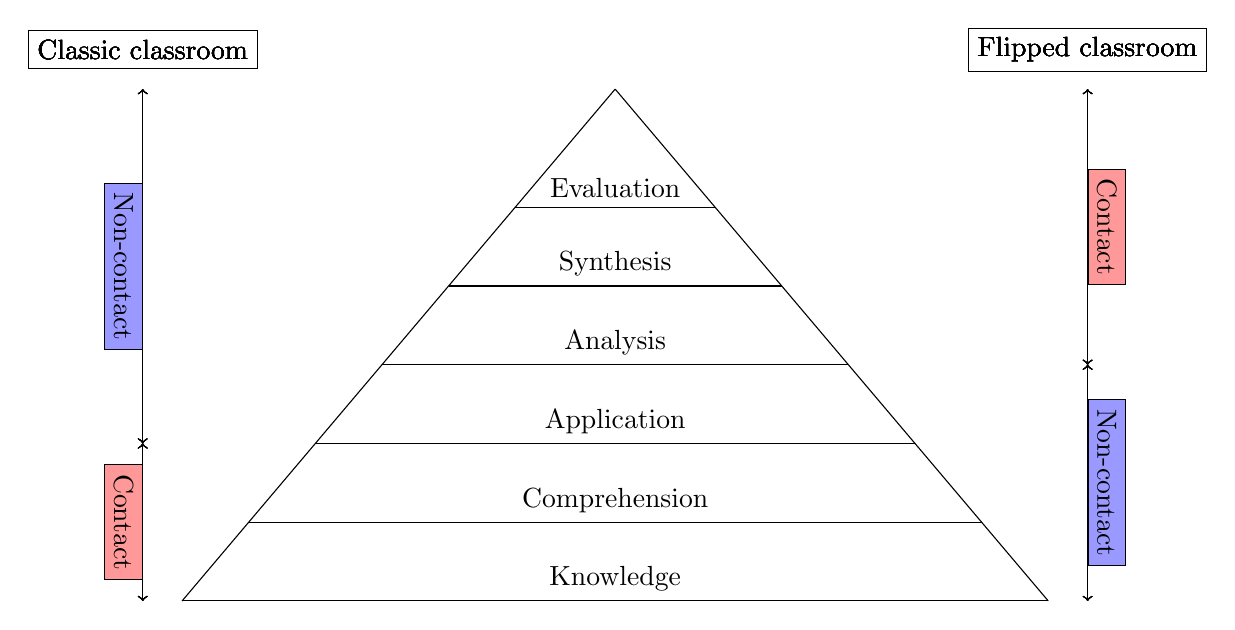
\begin{tikzpicture}
% Bloom's pyramid
\coordinate (A) at (-5.5,1) {};
\coordinate (B) at ( 5.5,1) {};
\coordinate (C) at (0,7.5) {};
\draw[name path=AC] (A) -- (C);
\draw[name path=BC] (B) -- (C);
\foreach \y/\A in {1/Knowledge,2/Comprehension,3/Application,4/Analysis,5/Synthesis,6/Evaluation} {
\path[name path=horiz] (A|-0,\y) -- (B|-0,\y);
\draw[name intersections={of=AC and horiz,by=P},
name intersections={of=BC and horiz,by=Q}] (P) -- (Q)
node[midway,above] {\A};

% Traditional contact time
\node at (-6, 8) [rectangle, draw] {Classic classroom};
\draw [<->] (-6,1) -- (-6,3) node [below, midway, rotate=-90, rectangle, draw, fill=red!40] {Contact};
\draw [<->] (-6,3) -- (-6,7.5) node [below, midway, rotate=-90, rectangle, draw, fill=blue!40] {Non-contact};
% Flipped classroom contact time
\node at (6, 8) [rectangle, draw] {Flipped classroom};
\draw [<->] (6,1) -- (6,4) node [above, midway, rotate=-90, rectangle, draw, fill=blue!40] {Non-contact};
\draw [<->] (6,4) -- (6,7.5) node [above, midway, rotate=-90, rectangle, draw, fill=red!40] {Contact};
}
\end{tikzpicture}
\end{center}
\caption{Bloom's taxonomy and contact time in classic versus flipped classrooms}\label{bloominaflippedclassroom}
\end{figure}

As will become clear a flipped classroom approach is suited to the teaching of this module facilitating quality learning and ensuring the achievement of the intended learning outcomes. I base this assertion on the three following points:

\begin{itemize}
\item \textbf{The body of literature}:

First of all it is evident that flipped classrooms can work in large classes, as indicated in \cite{bates_inverted_2012, deslauriers_improved_2011, gannod_using_2008, moravec_learn_2010}. Not only is this an appropriate approach for the class size but flipped classrooms have been shown to promote effective learning and achievement of relevant intended learning outcomes by students from a range of learning styles; see \cite{bartlett_flip_1995, bates_inverted_2012, deslauriers_improved_2011, moravec_learn_2010, noora_review_2013, pinder-grover_efficacy_2011}. Further to this research showing benefits there is also research that reassuringly shows that there are no reasons to believe that a flipped classroom would give \textit{worse} results \cite{frederickson_evaluating_2005}. Finally there is also evidence that flipped classrooms improve cooperation and innovation \cite{strayer_how_2012} as well as promoting inclusive environments \cite{lage_inverting_2000}.

\item \textbf{Feedback from previously taught courses}:

In my second portfolio I discussed some feedback I collected from a questionnaire distributed to my students at the end of a portion of a module I taught using a small amount of flipped classroom methodologies. I gaged that students seemed to be quite receptive to the various resources presented to them prior to lectures and as such I developed a new module (MAT013 delivered for the first time in the spring semester of 2013) that was delivered entirely using a flipped classroom and IBL pedagogy. I am very pleased to say that this was a resounding success. I base that conclusion on the performance of the students in their various assessments, end of module feedback questionnaires but also on numerous discussions held with the students throughout the module. Whilst some found the shift of responsibility and focus (from the teacher to the learner) difficult to master at the beginning, there seemed to be a quasi unanimous agreement at the end of the module that the students had empowered themselves to be better learners.

\item \textbf{Work carried out in the group project for this module \cite{anderson_understanding_2013}}:

Given that a flipped classroom requires student engagement in an exercise that they can ultimately choose to not engage in. Content delivery can be thought of as a form of formative assessment. Engagement with and perception of formative assessment was the particular focus of the group work for this PCUTL portfolio \cite{anderson_understanding_2013}. I will not present here the main findings of that study, a major aspect of which was the analysis of a questionnaire, however relevant to the current discussion is the following statement which was presented to participants:

\begin{quotation}
\textit{I am more likely to do homework if it is to be done before a lecture on the subject.}
\end{quotation}

The responses to this question were bi modal with some students being quite receptive and some being less receptive as shown in Figure \ref{morelikelytodohomeworkbeforelecture}.

\begin{figure}[htdp]
\begin{center}
\includegraphics[width=10cm]{./Images/morelikelytodohomeworkbeforelecture.pdf}
\end{center}
\caption{Responses to a statement relevant to flipped classrooms. (1: Strongly disagree; 2: Disagree; 3: Indifferent; 4: Agree; 5: Strongly agree)}\label{morelikelytodohomeworkbeforelecture}
\end{figure}

In general most of our responses seemed fairly similar when it came to innovative teaching and assessment methodologies. As stated in Chapter 1 of \cite{bryan_innovative_2006} by Gibbs this is most probably explained by students' resistance to methods of assessment that are new to them or that they feel might take more time. I certainly feel that this applies in the case of flipped classrooms given the previously cited literature as well as previous experience with students who all seem to engage well. Nevertheless, the main consideration I must make is that certain students will potentially not engage without incentive to the methodology and/or would not benefit from this pedagogical approach. I will discuss how I have planned to address this in the next section.
\end{itemize}

In the next section I will describe the delivery, assessment and feedback for CfM that not only fits in line with \cite{cardiff_university_cardiff_2013} but also fully allows for the creation of independent learners as prescribed by \cite{cardiff_university_way_2013}.

\subsection{Delivery, assessment and feedback}

A diagrammatic representation of the delivery of the module is shown in Figure \ref{CfMdelivery}.

\begin{figure}[htdp]
\begin{center}
\framebox{
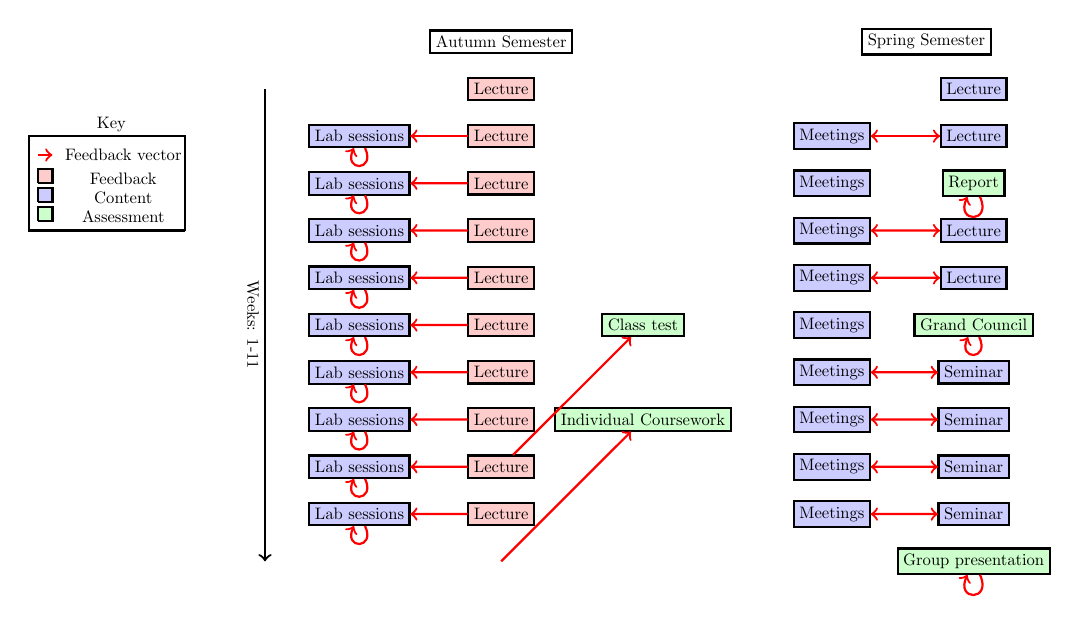
\begin{tikzpicture}[thick,scale=0.6, every node/.style={scale=0.6}]
\begin{scope}[xshift=-3cm, yshift=-3cm]
    \node at (-2.25, 3.25) {Key};
    % Color key
    \draw (-.7, 1) -- (-4, 1) -- (-4, 3) -- (-.7, 3) -- (-.7, 1);
    % Feedback
    \draw [fill=green!20] (-3.8, 1.2) -- (-3.8, 1.5) -- (-3.5, 1.5) -- (-3.5, 1.2) -- (-3.8, 1.2);
    \node at (-2, 1.3) {Assessment};
    % Content
    \draw [fill=blue!20] (-3.8, 1.6) -- (-3.8, 1.9) -- (-3.5, 1.9) -- (-3.5, 1.6) -- (-3.8, 1.6);
    \node at (-2, 1.7) {Content};
    % Assessment
    \draw [fill=red!20] (-3.8, 2) -- (-3.8, 2.3) -- (-3.5, 2.3) -- (-3.5, 2) -- (-3.8, 2);
    \node at (-2, 2.1) {Feedback};
    % Feedback direction
    \draw [red, ->] (-3.8, 2.6) -- (-3.5,2.6);
    \node  at (-2, 2.6) {Feedback vector};
\end{scope}
%------------ Weeks
\draw [->] (-2,1) -- (-2,-9) node [midway, below, rotate=-90] {Weeks: 1-11};


% ----------- Autumn
\node [rectangle, draw] at (3,2) {Autumn Semester};
% Draw lab session boxes
\node (week2) [rectangle, draw, fill=blue!20] at (0,0) {Lab sessions};
\node (week3) [rectangle, draw, fill=blue!20] at (0,-1) {Lab sessions};
\node (week4) [rectangle, draw, fill=blue!20] at (0,-2) {Lab sessions};
\node (week5) [rectangle, draw, fill=blue!20] at (0,-3) {Lab sessions};
\node (week6) [rectangle, draw, fill=blue!20] at (0,-4) {Lab sessions};
\node (week7) [rectangle, draw, fill=blue!20] at (0,-5) {Lab sessions};
\node (week8) [rectangle, draw, fill=blue!20] at (0,-6) {Lab sessions};
\node (week9) [rectangle, draw, fill=blue!20] at (0,-7) {Lab sessions};
\node (week10) [rectangle, draw, fill=blue!20] at (0,-8) {Lab sessions};
% Draw Lecture boxes
\node (lec1) [rectangle, draw, fill=red!20] at (3,1) {Lecture};
\node (lec2) [rectangle, draw, fill=red!20] at (3,0) {Lecture};
\node (lec3) [rectangle, draw, fill=red!20] at (3,-1) {Lecture};
\node (lec4) [rectangle, draw, fill=red!20] at (3,-2) {Lecture};
\node (lec5) [rectangle, draw, fill=red!20] at (3,-3) {Lecture};
\node (lec6) [rectangle, draw, fill=red!20] at (3,-4) {Lecture};
\node (lec7) [rectangle, draw, fill=red!20] at (3,-5) {Lecture};
\node (lec8) [rectangle, draw, fill=red!20] at (3,-6) {Lecture};
\node (lec9) [rectangle, draw, fill=red!20] at (3,-7) {Lecture};
\node (lec10) [rectangle, draw, fill=red!20] at (3,-8) {Lecture};
% Draw feedback arrows
\draw [red, ->] (lec2) -- (week2);
\draw [red, ->] (week2) to [out=-65, in=-115, looseness=6]  (week2);
\draw [red, ->] (lec3) -- (week3);
\draw [red, ->] (week3) to [out=-65, in=-115, looseness=6]  (week3);
\draw [red, ->] (lec4) -- (week4);
\draw [red, ->] (week4) to [out=-65, in=-115, looseness=6]  (week4);
\draw [red, ->] (lec5) -- (week5);
\draw [red, ->] (week5) to [out=-65, in=-115, looseness=6]  (week5);
\draw [red, ->] (lec6) -- (week6);
\draw [red, ->] (week6) to [out=-65, in=-115, looseness=6]  (week6);
\draw [red, ->] (lec7) -- (week7);
\draw [red, ->] (week7) to [out=-65, in=-115, looseness=6]  (week7);
\draw [red, ->] (lec8) -- (week8);
\draw [red, ->] (week8) to [out=-65, in=-115, looseness=6]  (week8);
\draw [red, ->] (lec9) -- (week9);
\draw [red, ->] (week9) to [out=-65, in=-115, looseness=6]  (week9);
\draw [red, ->] (lec10) -- (week10);
\draw [red, ->] (week10) to [out=-65, in=-115, looseness=6]  (week10);
% Highlight assessment
\node (ass1) [rectangle, draw, fill=green!20] at (6,-4) {Class test};
\node (ass2) [rectangle, draw, fill=green!20] at (6,-6) {Individual Coursework};
% Feedback loops for assessment
\draw [red, ->] (lec9) -- (ass1);
\draw [red, ->] (3, -9) -- (ass2);
% ----------- Spring
\begin{scope}[xshift=10cm]
\node [rectangle, draw] at (2,2) {Spring Semester};
% Draw lab session boxes
\node (week2) [rectangle, draw, fill=blue!20] at (0,0) {Meetings};
\node (week3) [rectangle, draw, fill=blue!20] at (0,-1) {Meetings};
\node (week4) [rectangle, draw, fill=blue!20] at (0,-2) {Meetings};
\node (week5) [rectangle, draw, fill=blue!20] at (0,-3) {Meetings};
\node (week6) [rectangle, draw, fill=blue!20] at (0,-4) {Meetings};
\node (week7) [rectangle, draw, fill=blue!20] at (0,-5) {Meetings};
\node (week8) [rectangle, draw, fill=blue!20] at (0,-6) {Meetings};
\node (week9) [rectangle, draw, fill=blue!20] at (0,-7) {Meetings};
\node (week10) [rectangle, draw, fill=blue!20] at (0,-8) {Meetings};
% Draw Lecture boxes
\node (lec1) [rectangle, draw, fill=blue!20] at (3,1) {Lecture};
\node (lec2) [rectangle, draw, fill=blue!20] at (3,0) {Lecture};
\node (lec3) [rectangle, draw, fill=green!20] at (3,-1) {Report};
\node (lec4) [rectangle, draw, fill=blue!20] at (3,-2) {Lecture};
\node (lec5) [rectangle, draw, fill=blue!20] at (3,-3) {Lecture};
\node (lec6) [rectangle, draw, fill=green!20] at (3,-4) {Grand Council};
\node (lec7) [rectangle, draw, fill=blue!20] at (3,-5) {Seminar};
\node (lec8) [rectangle, draw, fill=blue!20] at (3,-6) {Seminar};
\node (lec9) [rectangle, draw, fill=blue!20] at (3,-7) {Seminar};
\node (lec10) [rectangle, draw, fill=blue!20] at (3,-8) {Seminar};
\node (lec11) [rectangle, draw, fill=green!20] at (3,-9) {Group presentation};
% Draw feedback arrows
\draw [red, <->] (lec2) -- (week2);
\draw [red, <->] (lec4) -- (week4);
\draw [red, <->] (lec5) -- (week5);
\draw [red, <->] (lec7) -- (week7);
\draw [red, <->] (lec8) -- (week8);
\draw [red, <->] (lec9) -- (week9);
\draw [red, <->] (lec10) -- (week10);
% Highlight assessment
\draw [red, ->] (lec11) to [out=-65, in=-115, looseness=6] (lec11);
\draw [red, ->] (lec6) to [out=-65, in=-115, looseness=6] (lec6);
\draw [red, ->] (lec3) to [out=-65, in=-115, looseness=6] (lec3);
\end{scope}
\end{tikzpicture}
}
\end{center}
\caption{Delivery of content, feedback and assessment for CfM}\label{CfMdelivery}
\end{figure}

As can been seen in Figure \ref{CfMdelivery} the delivery of this module is dependent on the semester. Indeed CfM can be thought of in two parts:

\begin{enumerate}
    \item Autumn semester: acquisition of programming skills;
    \item Spring semester: use of programming skills in an entrepreneurial environment.
\end{enumerate}

\subsubsection{Autumn semester: acquisition of programming skills}

This semester will be taught in a constructivist framework \cite{jordan_approaches_2008} using a flipped classroom approach. Whilst traditional flipped classrooms imply students carry out work completely out of the classroom context (`at home'), as discussed previously the content delivery of a flipped classroom can be thought of as formative assessment and as such it is important to incentivise students to engage with the methodology (this is discussed in \cite{anderson_understanding_2013}). Keeping this in mind the following two approaches are going to be used:

\begin{itemize}
    \item Scheduled lab sessions;
    \item ``Tickables''.
\end{itemize}

The scheduled lab sessions (as depicted in Figure \ref{CfMdelivery}) occur before the lecture on a subject. Students will attend two lab sessions (over a period of three days) during which they will be required to tackle a set of problems. These problem sheeets are designed in such a way as to allow the students to construct their understanding of the programming concepts required to achieve the intended learning outcomes. Note that in \cite{anderson_understanding_2013} it was indicated that some students were more likely to  carry out formative assessment if there was a timetabled session for it as shown in Figure \ref{morelikelytodohwiftimetabled}. It can be seen that some students disagree with this statement. I believe that they are in fact indifferent to them: however as I am about to describe, the design of these timetabled slots take this possibility in to account, ensuring quality learning by students of a variety of learning styles.

\begin{figure}[htdp]
\begin{center}
\includegraphics[width=10cm]{Images/morelikelytodohwiftimetabled.pdf}
\caption{Responses by year of study to the statement: "I am more likely to do non marked homework if there is a timetabled slot for it". (1: Strongly disagree; 2: Disagree; 3: Indifferent; 4: Agree; 5: Strongly agree)}\label{morelikelytodohwiftimetabled}
\end{center}
\end{figure}

Often, when discussing flipped classrooms one immediately thinks of `videos' however this is not necessarily a requisite of a flipped classroom, all that is required is a shift in the locus of knowledge delivery \cite{robert_talbert_inverted_2013}. Nonetheless to ensure that learners of all types are catered for in what will be to them, a novel pedagogic environment; 110 short (less than 5 minutes) videos have been developed that not only explain certain concepts (whilst still leaving enough scope for self constructed learning) but also act as a feed forward mechanism \cite{conaghan_feedback_2009}.

The purpose of these lab sessions is to encourage constructivist learning \textbf{and not ``teaching''}. As such students will be encouraged to tackle problems independently. The following sequence of questions will be used by each tutor when a student is unable to carry out an exercise?

\begin{enumerate}
    \item Have you read the description in the lab sheet fully?
    \item Have you watched the video?
    \item Have you attempted to search for other resources?
\end{enumerate}

Of course, if a student is still unable to tackle a problem then the tutor will be most able to help.

As indicated in Figure \ref{CfMdelivery} there is a feedback loop taking place within the lab sessions. \textbf{At this point, the reader might be enquiring how tutors will be able to give feedback during the lab sessions (given the large number of students).} The methodology used is called `Tickables'. This is based on an approach by the same name used by Bath University. I attended a workshop organised by the HEA entitled: `Experiences of learning programming within a mathematics course'. The idea is that on each of the lab sheets, a certain number of questions are marked as `TICKABLE'. These questions are marked as pass/fail (`tick') in the lab sessions themselves by the tutors. Students who complete less than 80\% of their tickables will lose 10\% of their final mark for the module.

Importantly tutors are given some basic directions as to the marking of tickables:

\begin{itemize}
    \item The marking ('ticking') is to be done in class;
    \item To succeed at a tickable students must not necessarily succeed at doing it but more importantly spend a sufficient amount of time attempting to do it;
    \item Tutors are allowed a certain level of subjective judgement.
\end{itemize}

This allows tutors to give immediate feedback to students: `nearly there, you need to include something like this...' but also to receive feedback from students as to what they are having difficulty with. This is where the process as indicated in Figure \ref{CfMdelivery} is indeed `flipped'. As the lecturer I will obtain feedback from the tutors as to the points that need to be addressed in the lecture.

Furthermore students are encouraged during the lab sessions to work in groups. Figure \ref{peerinstruction} shows an example of this occurring when the student in the checkered shirt was able to explain a particular concept to a large number of students in his particular lab session.

\begin{figure}[htdp]
\begin{center}
\includegraphics[width=10cm]{./Images/peerinstruction.png}
\end{center}
\caption{Peer instruction in action: the student in the checkered shirt is explaining a concept to his peers.}\label{peerinstruction}
\end{figure}

As stated earlier, students who would rather work outside of the lab sessions are very welcome to. It is entirely imaginable and acceptable for a student to arrive at their first lab session having completed all their tickables, gets them checked by a tutor and simply leaves. This again ensures that most types of learners are catered for.

Given the break from the traditional pedagogies that the students will experience in the School of Mathematics and also to ensure that students feel that they receive sufficient contact time with me (an element that is of high importance on the National Student Survey which is in turn important with regards to \cite{cardiff_university_way_2013}) I have put in place official `office hours'. Whilst my door is always open to students I am often away from the office and also am not always available. Thus I have made clear to the students that I will be in my office during office hours solely for the purpose of giving feedback and/or addressing queries that might potentially arise due to certain students not being comfortable within my pedagogic approach.

Figure \ref{emailaboutofficehours} shows an email received from a student who has fully engaged with the process (having not only completed the tickables but the entire sheet before the first lab session). As can been seen I plan to use my office hours to address the needs for this particular student and potentially indicate further areas for him to explore.

\begin{figure}[htdp]
\begin{center}
\includegraphics[width=14cm]{Images/emailaboutofficehours.pdf}
\end{center}
\caption{A student that will make use of office hours}\label{emailaboutofficehours}
\end{figure}

Furthermore the nature of this class allows for a very clear evaluation of student comprehension by simply looking at their progress. Figure \ref{emailaboutlabsheet} shows an email exchange with a group of students who were working on a particular problem. Just by showing me their code I am able to give precise and relevant feedback.

\begin{figure}[htdp]
\begin{center}
\includegraphics[width=14cm]{Images/emailaboutlabsheet.png}
\end{center}
\caption{Giving precise feedback via email}\label{emailaboutlabsheet}
\end{figure}

Finding tutors for the large quantity of lab sessions (there will be 20 lab sessions a week) is in itself a challenge. In future years, to encourage peer learning \cite{crouch_peer_2001, falchikov_learning_2002}, students in their second year will be used as tutors however this is not possible as the course is running for the first time. As a result, various members of staff in the School of Mathematics have kindly given up their time to tutor the lab session this year.

This section of the course will be assessed through a class test at the mid point of the first term which will evaluate students' knowledge of Python. This has been difficult to put in place once again due to class size as it is desirable to have this class test in front of a computer to ensure that it fully assesses the corresponding intended learning outcome. In \cite{chamillard_evaluating_2000} it is shown that this is an appropriate approach of assessing programming ability. It is important to have a class test to ensure a balance of assessment methodologies as well as an appropriate evaluation of individual student abilities. In the literature concerns have been voiced trends to increase coursework assessment (due to increasing student numbers) \cite{gibbs_coursework_1997} which often give higher marks than tests or exams \cite{bridges_coursework_2002}.

After many discussions with members of the learning and teaching team within the School of Mathematics as well as with my mentor who is the director of our MSc programmes in Operational Research; it seems that there will be enough capacity within the School to assess all students in front of a computer. This is an effective and appropriate assessment of the first learning outcome for CfM.

The second method of assessment will be an individual coursework exercise. As for the class test, this is an effective and appropriate assessment of the second and third learning outcome for CfM (\cite{chamillard_evaluating_2000}). This coursework is meant to not only assess students ability to use Sage and LaTeX but also to prepare them for the independent work that will be required of them in the second semester.

To ensure that both these methods of assessment facilitate student learning I will give timely and relevant feedback as shown in Figure \ref{CfMdelivery} in line with the recommendations of \cite{gibbs_conditions_2004}.

Before describing the second semester of this module (recall Figure \ref{CfMdelivery}) I will describe the method of delivery of all relevant teaching materials (lab sheets, videos, handouts etc...). All documents are delivered via my personal website (\url{www.vincent-knight.com}) in a variety of formats (html, pdf and word). Delivering mathematical teaching content in multiple formats is notoriously difficult however it is a problem I addressed and solved in my previous portfolio. All videos for this module are delivered via YouTube using an `unlisted format' so that only students with the relative urls can find them (this links are distributed via the lab sheets). Figure \ref{videoviews} shows the top views of my YouTube channel from the first week of CfM. This shows that students are not only watching these videos but on some occasions watching them multiple times.

\begin{figure}[htdp]
\begin{center}
\includegraphics[width=9cm]{./Images/videoviews.png}
\end{center}
\caption{Some viewing statistics of the videos for this course}\label{videoviews}
\end{figure}


An appendix including links to all my teaching materials is available in this portfolio. This methodology ensures that students can access all of the materials on any platform and/or operating system. Finally, delivery through electronic resources has been described as an appropriate methodology for my pedagogic approach \cite{kellogg_developing_2009} and there is even evidence showing that students prefer this method of delivery \cite{brown_student_2004}.

\subsubsection{Spring semester: use of programming skills in an entrepreneurial environment}

I will attempt to keep this section short as the Spring semester is the topic of my mentor peer review however here is a brief summary:

\begin{itemize}
\item Students will be organised into groups of 4. These groups will be called `companies' and entrepreneurial themes will be present throughout the spring semester.
\item Companies will agree on a structure which will include a `project manager' and a `secretary'.
\item The roll of the secretary is to ensure that the company meets twice a week with minutes collected.
\item Companies will have as a goal to identify a particular mathematical `product' that can be created using the programming tools acquired in the autumn semester.
\end{itemize}

As shown in Figure \ref{CfMdelivery} there is a limited amount of contact time in this part of the module with one session (lecture or seminar) timetabled a week. At the beginning of the term this will be used by the entrepreneurial team from the Cardiff University students' union (Figure \ref{stuartemail} shows an ongoing email discussion ensuring that the assessment schemes for this are appropriate) as well as the library to present valuable skills to the students. The seminars will be used to expose students to further aspects of programming such as other programming languages and/or some research that is being done in the school. This later aspect fully ensures that students are exposed to research lead teaching.

\begin{figure}[htdp]
\begin{center}
\includegraphics[width=12cm]{./Images/stuartemail.png}
\end{center}
\caption{Ensuring the appropriateness of assessment}\label{stuartemail}
\end{figure}

The work carried out this semester will be assessed using group coursework (three week report) as well as a group presentation. I feel that the three week report (although summative) plays more of of a formative role to ensure that students are on the right track (although it is also appropriate to assess the third learning outcome of CfM). The group presentation is an appropriate assessment methodology for the fourth learning outcome of CfM.

I feel that these approaches to pass entrepreneurial skills on to the students is in line with the literature \cite{solomon_examination_2007}. Furthermore these are in line with the `embedded' recommendations made in \cite{evas_embedding_2013} (another PCUTL group project) where a similar approach was suggested: it was suggested that students form `research groups' and write research proposals.

In the next section I will briefly discuss how this module fits within the wider programme of study on offer at the School of Mathematics.

\section{Computing for Mathematics as part of a programme}

In \cite{elton_are_1998} the opinion is given that degree programmes in the UK are becoming more diversified and `standards are going sideways'. With the CfM module I would argue that the School of Mathematics is indeed diversifying their degree but as suggested previously this is a competitive diversification as it will lead to better mathematics graduates:

\begin{itemize}
\item A better understanding of what it is to be a mathematician;
\item An ability to carry out mathematical research both independently and in a group environment;
\item A competitive advantage in a competitive employment market.
\end{itemize}

Importantly, this module will allow for better learning by a range of undergraduates throughout their programme at the School of Mathematics. Indeed, I am in discussion with the leaders of second and third year modules to ensure that further programming will be embedded and/or used throughout the curriculum. On a personal level I will find the teaching of my third year Game Theory module to offer greater interactivity and understanding once all students have a comfortable set of programming skills.

This module was designed using a form of constructive alignment \cite{biggs_teaching_2011}. Indeed, as stated previously, it began with the assertion that modern mathematics graduates needed to know how to program. This would be assessed through their ability to write code but also through their ability to work with others which is in line with \cite{cardiff_university_way_2013}. The teaching and learning activities were designed to ensure students would be able to attain the learning outcomes, and basing these on previous experiences as well the evidence from the literature, a novel pedagogic approach is being used. Specific consideration has been given to the contact and non contact time given the flipped classroom approach (recall Figure \ref{CfMdelivery}).

The assessment of the effect that this module has on the entire programme of study will be an ongoing study as students go through the years. I hope to make the learning of computing by mathematics students an area of investigation for my fourth PCUTL module but also for my future educational research activities.

In the next section I will briefly carry out a critique of the group project I carried out as part of this module of PCUTL and importantly place my experience gained through this group project in a valuable setting for my future teaching.

\section{Discussion of group project}

I will not in the section discuss the findings of the group project but more so my experience as a student working within a group. In \cite{davies_groupwork_2009} a wide range of advantages of group work are discussed which not only include pedagogic arguments but also certain pragmatic ones such as the fact that group work allows for an efficient way of handling large class sizes. The paper mainly discusses various difficulties linked to group work and how to address them:

\begin{itemize}
    \item The free-rider problem;
    \item The sucker effect problem;
    \item Groupwork and ethnic mix;
    \item The social dilemma problem.
\end{itemize}

In our particular group project, whilst we did have a variety of differing opinions I would not say that any of the four above problems where specifically difficult to deal with.

I feel that the minor difficulties were indeed kept minor due to the maturity of the group members. This will not necessarily be the case with the group work planned for first year undergraduates in CfM and as such I will be sure to take on board the pre existent recommendations throughout the literature \cite{bartlett_flip_1995, davies_groupwork_2009}.

One particular aspect that will hope help avoid the `sucker effect' is how to incentivise students to ensure that they all work equally. I have discussed this already in my previous portfolio. In particular I have since implemented a methodology based on a game theoretic approach. I have already discussed the advantages and disadvantages of my proposed approach but in the near future I plan to investigate this further and importantly justify how I feel that this approach could contribute to the literature on the subject \cite{lejk_survey_1996}. My approach is not the one that we chose to use within our group. The main reason for this was to ensure a fair workload amongst the group. My contribution included the majority of the statistical content analysis content for the project and so after some discussion it was decided to share the rest of the work.

Another aspect that was of interest during the group project was the use of technology. I have already widely discussed my use of technology in the classroom and it is something I am fairly confident with. However, it was nice to see that we were able to use Google Drive \cite{google_go_2012} in an efficient way to put our project report and slides together as shown in Figure \ref{repoongoogledrive}.

\begin{figure}[htdp]
\begin{center}
\includegraphics[width=14cm]{./Images/repoongoogledrive.png}
\end{center}
\caption{Discussing our document in real time on Google Drive}\label{repoongoogledrive}
\end{figure}

Interestingly, whilst most of us seemed quite happy with this as a tool and in particular thought it allowed us to work efficiently as a group, there was a member of our group who voiced certain aspects that were not to their liking. On a similar note I have blogged about the fact that Google Drive is not suitable for Mathematical work \cite{knight_using_2012} and as such I have already planned to match the second intended learning outcome of CfM with writeLaTeX (\url{www.writelatex.com/}), a cloud based service similar to Google Drive.

Just before the group presentation some of our group members where not in the UK which made a practice run of the presentation difficult. One option would have been to use a VOIP service such as google hangouts or skype, however this was a busy time of year and as such it was difficult to find a mutually convenient time. As a solution I created a screencast of the talk and uploaded it to YouTube \cite{vincent_knight_understanding_2013}. Importantly, as we did not necessarily know if we were happy with the presentation I uploaded it as an `unlisted' video so it can not be found by anyone without the correct url. This was viewed by the group which allowed us to discuss certain aspects of the talk.

\section{Conclusions}

I have put together a well designed new module that fits within the programme of study at the School of Mathematics. Importantly the delivery, assessment and feedback has been carefully thought of and ensures that students from a wide range of learning styles should be able to effectively reach the desired learning outcomes. Whilst my methodologies are not as extreme as other proven techniques \cite{davis_how_2013} they still will require careful monitoring and evaluation.

In the future I plan to undertake the fourth module of PCUTL as well as continue to engage with educational literature (ideally contributing myself). Whilst, I have discussed a wide range of literature that gives evidence to the benefits of flipped classrooms there is still research that can and must be done. Some of the `missing research' has been discussed at \cite{weinberg_reviewing_2013}: pointing out that most studies show progression of learning but not on the same student group.  I hope to concentrate my education research on the subject of how mathematics students learn to program. In \cite{crawford_university_1998}, a paper written in 1998 student perceptions of mathematics are presented. I would very much like to carry out a similar study on a longitudinal scale. In \cite{crawford_university_1998} no mention of computing was made. It would be interesting to see if things have changed since but also if students' perceptions change over their time spent at Cardiff university.

Given the novel nature of CfM and my role as module leader I could use module four of PCUTL to investigate the above but also examine, critique and improve my delivery of CfM based on feedback from students as well as novel educational research.

I plan to continue my engagement with the educational research community. I am in talks with the director of Learning and Teaching at the School of Mathematics to organise a regular reading group meeting. With my mentor I am also planning a workshop entitled `Workshop on Innovations in HE Mathematics Teaching'. This is being planned with the HEA and as well as having myself and others discuss flipped classrooms will have Dana Ernst and Theron Hitchman from the US visiting to present on Inquiry Based Learning.

Furthermore I feel that I continue to encourage the participation in higher education to students of all backgrounds and abilities. This is ensured through my role as chair of the OR society working group: OR in schools. I also continue to partake in various outreach activities. Furthermore, by the choice of open source languages as the pillar of CfM I ensure that students who want to introduce themselves to the language on their own machine will not need to be able to afford it.

Given that this portfolio concludes the `compulsory' section of PCUTL I would like to end with some words regarding the process. Whilst, it has taken a ferocious amount of my time I am so extremely glad of the opportunity of going through it. It has opened my eyes to the world of pedagogic research and I hope has allowed me to reflect and improve my teaching and learning. I look forward to the opportunity to be able to mentor someone through the process one day. I also hope that some of the materials on the PCUTL section of my personal website might be helpful to mathematicians going through the process in the future. This is an extremely valuable process, and one that is perhaps not given enough support as it should be in certain areas. I feel that this will change  in years to come as more members of the teaching community at Cardiff go through PCUTL.

I will leave this essay with the following saying (I have found far too many different claims of origin to include them here):

\begin{center}
\textit{Tell me, I'll forget. Show me, I'll remember. Involve me, I'll understand.}
\end{center}

\newpage
\bibliographystyle{plain}
\bibliography{educationresearch.bib}
\end{document}
